\chapter{Graph Signal Dictionary Learning}
\section{The dictionary learning improvement under smoothness constraints}
\label{sec:DL}
As we previously hinted, in the work of Thanou, Shuman and Frossard the focus was on learning the parametric functions ($kernels$) through which it was possible to reconstruct the graph signal. Moreover, in their work they modelled the graph signal as a combination of overlapping local patterns, describing localized events on the graph which can appear in several vertices. This representation of the graph signal brought to a representation of the dictionary structure as a concatenation of subdictionaries, which are polynomials of the graph Laplacian. Under this assumption they then learned the coefficients of the kernels through a numerical optimization.

\subsection{The dictionary structure and main assumptions}
The dictionary structure we used, presented in \cite{Thanou2014}, is in the following form: we designed a graph dictionary $\mathcal{D} = [\mathcal{D}_1, \mathcal{D}_2,\dots,\mathcal{D}_S]$, or a concatenation of a set of $S$ subdictionaries, as:
\begin{equation}
  \mathcal{D}_s = \hat{g_s}(\mathcal{L}) = \rchi (\sum_{k=0}^K \alpha_{sk}\Lambda^k)\rchi^T =   \sum_{k=0}^{K} \alpha_{sk}\mathcal{L}^k
\end{equation}
where $\hat{g_s}$ is the pattern (\textit{the kernel}) of the subdictionary $\mathcal{D}_s$ and where the atom given by the $n^{th}$ column of subdictionary $\mathcal{D}_s$ is equal to $\frac{1}{\sqrt{N}}T_ng_s$, the translation operator defined in \autoref{eq:translation} divided by the constant $\frac{1}{\sqrt{N}}$.\\
However, despite the polynomial constraint guarantees the localization of the atoms in the vertex domain, it does not provide though any information about the spectral representation of the atoms. The two matrix inequalities already listed in \autoref{eq:overallProblem} take it into consideration:
\begin{align}
  0 \preceq \text{ } &\mathcal{D}_s \preceq cI, \quad \forall s \in \{1,2,\dots , S\},  \label{eqn:boundness}\\
  &\text{and}\\
  (c-\epsilon)I \preceq &\sum_{s=1}^{S}D_s \preceq (c+\epsilon)I \label{eqn:spectrum}
\end{align}
\autoref{eqn:boundness} accounts for the fact that our kernels are nonnegative and uniformly bounded by a given constant $c$ (which we will further suppose equal to 1), while \autoref{eqn:spectrum} accounts for the fact that the signals we consider usually contain frequency components spread across the entire spectrum and so the kernels should cover it as well. These two spectral constraints together contribute to increase the stability of the dictionary. On the other hand, it might be noted that the constraint in \autoref{eqn:spectrum}  should not be considered in the case of one single kernel, obviously, since imposing that the sum of all kernels has to stay around $1$ would give the trivial solution $g(\lambda) = 1 \text{  } \forall \lambda$\\.

We finally underline the fact that for the design of the dictionary the eigenvectors used are the ones from the normalized graph Laplacian (and not the unnormalized one), since this configuration revealed to be more suitable for our bodywork.

\section{The dictionary learning algorithm under smoothness constraints}
With these basis we therefore implemented a dictionary learning algorithm based on the one presented in \cite{Thanou2014} in order to add the smoothness priors. As previously mentioned, we can cast the general problem as the following optimization problem:
\begin{align}
  \underset{\small{\alpha \in \R^{(K+1)*S}, \text{ } X \in \R^{SN \times N}}}{\argmin} &||Y-\mathcal{D}X||^2_F + \mu ||\alpha||_2^2 \label{eq:objDictionary}\\
  \text{subject to} \quad &||x_m||_0 = T_0, \quad \forall m \in \{1,\dots,M\} \notag \\
  &\mathcal{D}_s = \sum_{k=0}^{K}\alpha_{sk}^k, \quad \forall s \in \{1,2,\dots,S\} \notag \\
  &0 \preceq \text{ } \mathcal{D}_s \preceq cI, \quad \forall s \in \{1,2,\dots , S\},\notag \\
  &(c-\epsilon)I \preceq \sum_{s=1}^{S}\mathcal{D}_s \preceq (c+\epsilon)I \notag
\end{align}
with:
\begin{itemize}
\item $\mu$ being a coefficient that should be enough guarantee the stability of the solution while preserving large values in the polynomial $\alpha$s;
\item $x_m$ corresponding to the $m^{th}$ column of the sparsity matrix $X$;
\item $T_0$ being the sparsity level of the coefficient of each signal;
\item $l_0$ being norm term, one time more standing for the sparsity need we already manifested.
\end{itemize}

Since the optimization problem is non convex, there is the need to approximate it by the alternation of two optimization subproblems that are convex, namely the sparse coding and the dictionary update step.\\

The sparse coding step aims at learning the sparsity matrix $X$ solving
\begin{equation}
  \argmin_{X} ||Y - \mathcal{D}X||^2_F \qquad \text{subject to} \quad ||x_m||_0 \leq T_0,
\end{equation}
and it is solved using the \gls{omp} method, an iterative greedy algorithm that at each step selects the element in the dictionary that is best correlated with the signal residual part; it subsequently produces a new estimation through the projection of the signal onto the dictionary elements that have already been selected. This method admits simple and fast implementation and it has been proven that his error on the approximation is only a small factor worse than the minimal error obtained through a non-sparse representation. \cite{Tropp2004}.\\

On the other side, the dictionary update step aims at finding the polynomial coefficients of the kernels by minimizing
\begin{equation}
  \underset{{\alpha \in \R^{(K+1)S}}}{\argmin} ||Y - \mathcal{D}X||^2_F + \mu||\alpha||_2^2
\end{equation}
subject to the remaining constraints in \autoref{eq:objDictionary}

To this main problem we then added the smoothness prior through the two different implementations we already presented in \autoref{sec:2implementations}, the first one trying to insert the smoothness assumption inside the objective function of the dictionary update step, while the second one focusing on adding a smoothness prior in the constraints of the optimization function.

\subsection{Smoothness prior in the objective function}
We remember the equations \ref{eq:polynom}, and we reformulate them as
\begin{equation}
  g(\lambda) = \sum_{k=0}^K\alpha_k \lambda^k = \sum_{n=0}^N\gamma_n \lambda^n \times \sum_{m=0}^M  \beta_m \lambda^m
  \label{eq:giLambda}
\end{equation}
With $h(\lambda) = \sum_{n=n}^N \gamma_n \lambda^n$ and $(\lambda - \lambda_M)(\lambda - \lambda_{M-1})\cdot_{\dots}\cdot (\lambda - \lambda_{M - N +1})$ being the two sub-polynomials in which \autoref{eq:giLambda} has been decomposed. Between these, $h(\lambda)$ represents the polynomial with the unknown coefficients to be found, while the polynomial in the unknown $\beta$ is the one obtained from imposing the highest eigenvalues as roots of the general polynomial \ref{eq:giLambda}.\\
In particular, what we do in order to retrieve them is to generate $V$, a Vandermonde matrix with the root eigenvalues of the Laplacian raised to the powers of the kernel polynomial and impose that the vector of $\beta_m$ coefficients we want is one of the vectors of the nucleus of $V$:
\begin{equation}
  V=
  \begin{bmatrix}
    1 & \lambda_{N-M+1} & \lambda_{N-M+1}^2 & \dots & \lambda_{N-M+1}^K\\
    1 & \lambda_{N-M+2} & \lambda_{N-M+2}^2 & \dots & \lambda_{N-M+2}^K\\
    \vdots & \ddots     &                   & \dots & \vdots\\
    1 & \lambda_N &       \lambda_N^2       & \dots & \lambda_N^K\\
  \end{bmatrix}
  , \qquad B=
  \begin{bmatrix}
    \beta_0\\
    \beta_1\\
    \vdots\\
    \beta_K
  \end{bmatrix}
\end{equation}
\begin{equation}
  \text{and} \qquad \textbf{V}\cdot \textbf{B} = \textbf{0}
\end{equation}

With $N$ being in this case the number of eigenvalues of $\mathcal{L}$.\\
In the case of the heat kernel, the function does not exactly go to 0 in the last eigenvalues considered, but it stays a little bit above it, that is why we relaxed this condition requesting the final $\lambda$s to be root of a polynomial with a vertical indicative offset. The following results show how this procedure is still a good improvement in such a way that we could use this approach to better model general low frequency kernels in more precise ways than simply asking them to go directly to 0.

Since we deal with the optimization problem in \autoref{eq:objDictionary} through \gls{lmi} tools, we try to model the vector containing the kernel coefficients in such a way that the structure itself already holds the information regarding the composition of the two sub polynomials. To do so, we multiply the two sub polynomials among each other without resolving the equation with known $\beta$, but leaving them as unknown, in such a way that the behavior of the overall polynomial emerges. We thus obtain the structure that every $\alpha$ coefficient should have in order to transmit the smoothness prior to the objective function. Namely:
\begin{equation}
  \begin{split}
    \sum_{n=0}^N\gamma_n \lambda^n \times \sum_{m=0}^M \beta_m \lambda^m &= (\beta_0  \gamma_0)\lambda^0   + (\beta_0 \gamma_1 + \beta_1 \gamma_0)\lambda + \dots + \\
    &(\beta_0 \gamma_N + \beta_1 \gamma_{N-1} + \dots + \beta_N \gamma_0)\lambda^N + \dots + \\
    &(\beta_1 \gamma_N + \beta_2 \gamma_{N-1} + \dots + \beta_{N+1} \gamma_0)\lambda^{N+1} + \dots +\\
    &(\beta_{N} \gamma_{N} + \beta_{N+1} \gamma_{N-1} + \dots + \beta_{M} \gamma_0)\lambda^{M} + \\
    &(\beta_{N+1} \gamma_{N} + \dots + \beta_{2N + 1} \gamma_1)\lambda_{M+1} + \dots +\\
    &(\beta_M \gamma_N)\lambda^{K}
  \end{split}
  \label{eq:sviluppo}
\end{equation}
Once we obtained it, we insert this new information about the kernels structure in the optimization objective function, where now the alpha vector has a reduced number of unknowns that have to be found. With the problem set in this way we can thus analyse the new results we obtain.

\subsection{Smoothness prior in the problem constraints}
Another approach to the problem is based on inserting this smoothness prior in the constraints of the optimization function. On one side this choice should be discarded in favour of the first approach, since adding other constraints to our already ill posed problem could add more non-desired complexity; on another side this choice could reveal motivated by the fact that the control over the behavior of the optimization algorithm is in this way more verifiable than in the previous case, in which a black-box-stile coefficients vector detains all the smoothness priors. In this case the constraint added is the imposition that the Vandermonde matrix, obtained selecting only the last $M$ high-frequency eigenvalues in the graph Laplacian, should give a null vector when multiplied by the vector of the alpha coefficients. If $N$ is the total number of nodes in the considered graph, then we have:
\begin{equation}
  \begin{bmatrix}
    1 & \lambda_{N-M} & \lambda_{N-M}^2 & \dots & \lambda_{N-M}^{K} \\
    1 & \lambda_{N-M+1} & \lambda_{N-M+1}^2 & \dots & \lambda_{N-M+1}^{K} \\
    \vdots & & \\
    1 & \lambda_P & \lambda_P^2 & \dots & \lambda_N^K \\
  \end{bmatrix}
  \begin{bmatrix}
    \alpha_0 \\
    \alpha_1 \\
    \vdots \\
    \alpha_K
  \end{bmatrix}
  =
  \begin{bmatrix}
    0\\
    0\\
    \vdots\\
    0
  \end{bmatrix}
\end{equation}
\subsection{The optimization algorithm}
The final optimization algorithm is described by the pseudocode in the algorithm \ref{alg:pseudocode1}:
\begin{algorithm}[b]
  \begin{algorithmic}[1]
    \Procedure{initialization}{}
      \State $Y \gets \text{Signal samples set}$
      \State $T_0\gets \text{Target sparsity}$
      \State $K \gets \text{Polynomial degree}$
      \State $S \gets \text{Number of subdictionaries}$
      \State $iterNum \gets \text{Number of iterations}$
      \State $\mathcal{D} \gets \text{Initial dictionary computed thirugh random kernels}$
    \EndProcedure
    \For{$i=1,2,\dots, iter$}
      \Procedure{Sparsity step}{}
        \State \text{Scale each atom in $\mathcal{D}$ to a unit norm}
        \State $X \gets \text{Sparsity estimation with \gls{omp}}$
        \State{Rescale $X$ and $\mathcal{D}$ to recover the polynomial structure}
      \EndProcedure
      \Procedure{Dictionary learning step}{}
        $\alpha \gets \text{kernels estimation through sdpt3}$
      \EndProcedure
      \Procedure{Dictionary update step}{}
        \State $\mathcal{D} \gets \sum_{k=0}^K \alpha_k \mathcal{L}^k$
      \EndProcedure
    \EndFor
  \end{algorithmic}
  \caption{Parametric dictionary learning on graph with smoothness priors}
  \label{alg:pseudocode1}
\end{algorithm}

\section{Results}
\label{sec:dataGen}
\subsection{Data Generation}
The datasets used in the experiments are composed by a signal $Y$, an adjacency matrix $W$ and the comparison kernels used after the algorithm execution to verify the quality of the results. The signal $Y$ is obtained as the repetition of $2000$ samples randomly generated by a uniform distribution, the graph manifold onto which the signal is structured has $30$ nodes (for simplicity reasons) while the edges that are elements of the weight matrix $W$ are generated from the gaussian function
\begin{equation}
  w_{ij} = e^{-\frac{||x_i - x_j||_2^2}{2\sigma^2}}
\end{equation}
following the approach in \cite{Kalofolias2016}. At the same time, the kernel coefficients we generated as ground truth values come respectively:
\begin{itemize}
  \item form the Taylor expansion for the heat kernels
\end{itemize}
\begin{equation}
  \hat{g(\lambda)} \approx e^{-2\lambda}
\end{equation}
\begin{itemize}
  \item from one of the synthetic kernels used in the dataset from \cite{Thanou2014}. In that work they use a dictionary resulting from a concatenation of 4 subdictionaries, each of them being a $20^{th}$ order polynomial of the graph Laplacian and capturing one of the four constitutive components of their signal class.
\end{itemize}

The number of iterations we apply in this first part of the work is $50$, as we found it is a good value for the algorithm to properly converge to a minimum, while the value of $\epsilon$ for the spectral boundaries in \autoref{sec:DictionaryLearningSection} has been set to $0.2$. Moreover, we assume the sparsity coefficient $T_0$ to be equal to $4$ and the parameter $\mu$ to be $10^{-4}$.

We use the \textit{sdpt3} solver in the \textit{yalmip} optimization toolbox to solve the quadratic problem and, in order to directly compare the methods here described, we always use the \gls{omp} optimization criteria for the sparse coding step.

Finally, the average normalized approximation error we examine in the results is estimated by:
\begin{equation}
  \frac{1}{|Y_{test}|}\sum_{m=1}^{|Y_{test}|}\frac{||Y_m - \mathcal{D}X_m||_2^2}{||Y_m||^2}
\end{equation}
with $|Y_{test}|$ being the cardinality of the testing set.

\subsection{First approach: smoothness in the structure}
Results are promising, especially from a computational time point of view. The experiments have been repeated several times, in order to be able to claim the stability of the algorithm and show a stable trend.

The two main metrics we analyse for the performance of the algorithm are the reproduction error and the computational time taken by the optimization step, in the algorithm named as $CPUTime$.

\begin{table}[htbp]
  \centering
  \begin{tabular}{c|c|c}
    \multicolumn{1}{c|}{\textbf{Iteration number}} &
    \multicolumn{1}{c}{\textbf{Original algorithm}} &
    \multicolumn{1}{|c}{\textbf{Smoothness assumption}}\\
    \hline
    1 & 0.0251 & 0.0263\\
    2 & 0.0252 & 0.0260\\
    3 & 0.0250 & 0.0262\\
    4 & 0.0252 & 0.0262\\
    5 & 0.0252 & 0.0261\\
    \textbf{Average} & 0.02514 & 0.02616\\
  \end{tabular}
  \caption{Reproduction error comparison for the Heat kernel dataset}
  \label{tab:errorHeat_struct}
\end{table}

\begin{table}[htbp]
  \centering
  \begin{tabular}{c|c|c}
    \multicolumn{1}{c|}{\textbf{Iteration number}} &
    \multicolumn{1}{c}{\textbf{Original algorithm}} &
    \multicolumn{1}{|c}{\textbf{Smoothness assumption}}\\
    \hline
    1 & 0.0213 & 0.0220\\
    2 & 0.0214 & 0.0220\\
    3 & 0.0215 & 0.0220\\
    4 & 0.0212 & 0.0221\\
    5 & 0.0215 & 0.0220\\
    \textbf{Average} & 0.02138 & 0.0220\\
  \end{tabular}
  \caption{Reproduction error comparison for the Thanou et al. kernel dataset}
  \label{tab:errorDorina_struct}
\end{table}

The two tables \ref{tab:errorHeat_struct} and \ref{tab:errorDorina_struct} list the reproduction errors for $5$ sample trials using both datasets and comparing the effect of the smoothness over the learning quality. As can be seen, adding the smoothness prior does not bring automatically to a better reproduction; this is probably due to the fact that the definition of smooth kernel is not completely rigorous in describing "how much" the kernel goes to $0$, thus we have to accept a margin of uncertainty in forcing the final smoothness part. The variation is anyway contained, such that it cannot be considered as properly worsening the dictionary learning.\\

On the other hand, this prior allows us to observe an improvement in the computational cost of the algorithm, here measured by $CPUTime$ and shown in the table \ref{tab:CPUTime_struct}. The results are promising since one of the next steps in this work can focus of the learning of high dimensional graphs, in which computational cost reduction is even more important. From this point of view we can thus state that adding the smoothness prior brings a significative advantage to the learning procedure.

\begin{table}[htbp]
  \centering
  \begin{tabular}{c|c|c}
    &
    \multicolumn{1}{c}{\textbf{No smoothness assumption}} &
    \multicolumn{1}{|c}{\textbf{Smoothness assumption}}\\
    \hline
    \textbf{Heat Kernel dataset} & 0.9334 s & 0.1001 s\\
    \textbf{Thanou et al. dataset} & 0.1661 s & 0.0989 s\\
  \end{tabular}
  \caption{Computational cost comparison for the Heat kernel and the Thanou et al. kernel dataset}
  \label{tab:CPUTime_struct}
\end{table}

The learning procedure behaves overall well, as depicted by the figures \ref{fig:kernelHeat_struct} and \ref{fig:kernelDorina_struct}, where the learned kernels are shown, as also in \autoref{fig:alphaHeat_struct} and \autoref{fig:alphaDorina_struct}, where the values of the kernel coefficients can be seen, as well as how the smoothness prior guarantees that the coefficients follow the original ones in a more faithful way.

\begin{figure}
  \begin{minipage}[c]{.5\textwidth}
    \centering
    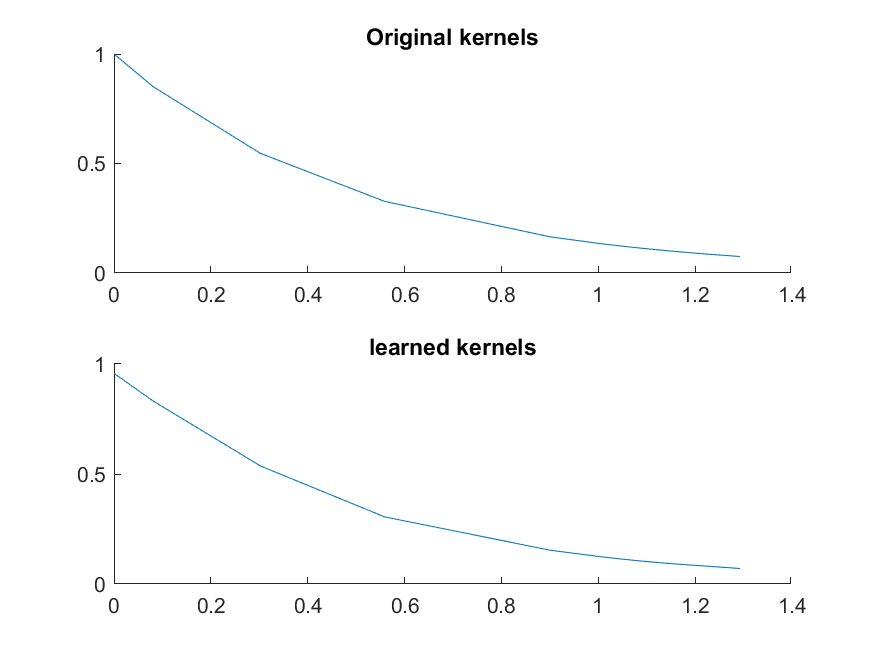
\includegraphics[width = \textwidth]{kernelHeat_noSmoothness_struct.png}
  \end{minipage}
  \begin{minipage}[c]{.5\textwidth}
    \centering
    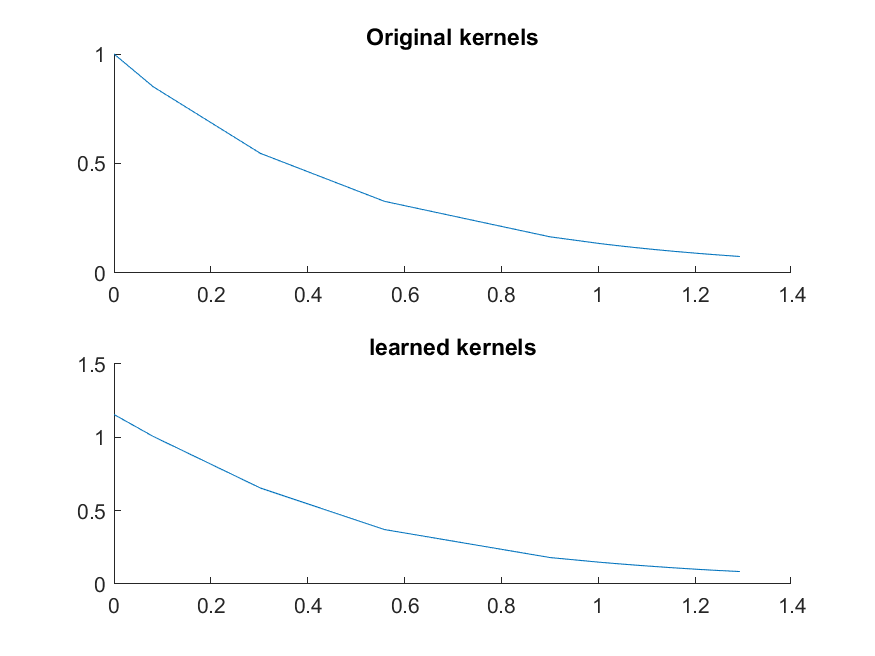
\includegraphics[width = \textwidth]{kernelHeat_Smoothness_struct.png}
  \end{minipage}
  \caption{Comparison between kernels without and with smoothness prior. Heat kernel dataset}
  \label{fig:kernelHeat_struct}
\end{figure}

\begin{figure}
  \begin{minipage}[c]{.5\textwidth}
    \centering
    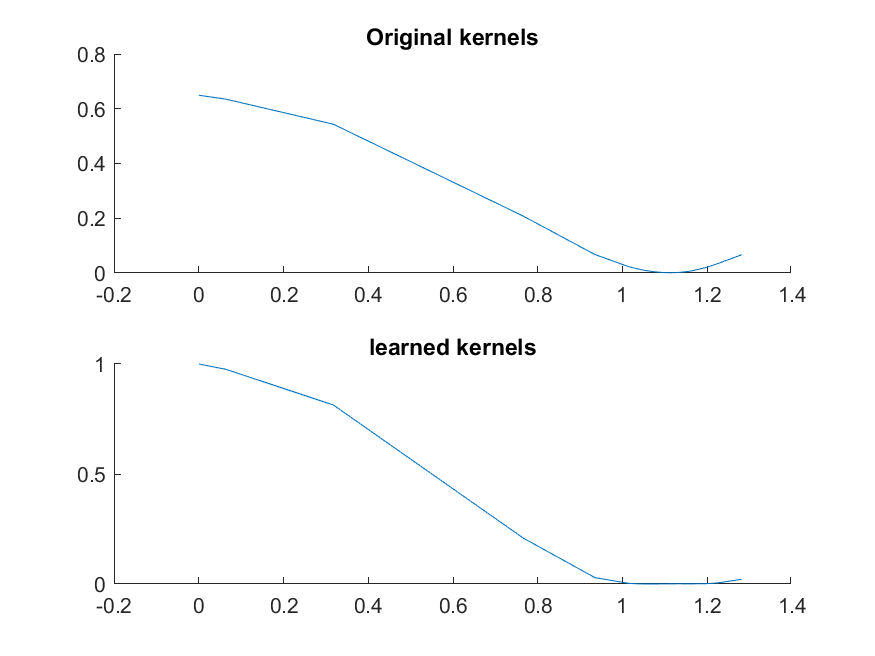
\includegraphics[width = \textwidth]{kernelDorina_noSmoothness_struct.png}
  \end{minipage}
  \begin{minipage}[c]{.5\textwidth}
    \centering
    \includegraphics[width = \textwidth]{kernelDorina_smoothness_struct.png}
  \end{minipage}
  \caption{Comparison between kernels without and with smoothness prior. Thanou et al. kernel dataset}
  \label{fig:kernelDorina_struct}
\end{figure}

\begin{figure}[htbp]
  \centering
  \begin{minipage}[c]{.85\textwidth}
    \centering
    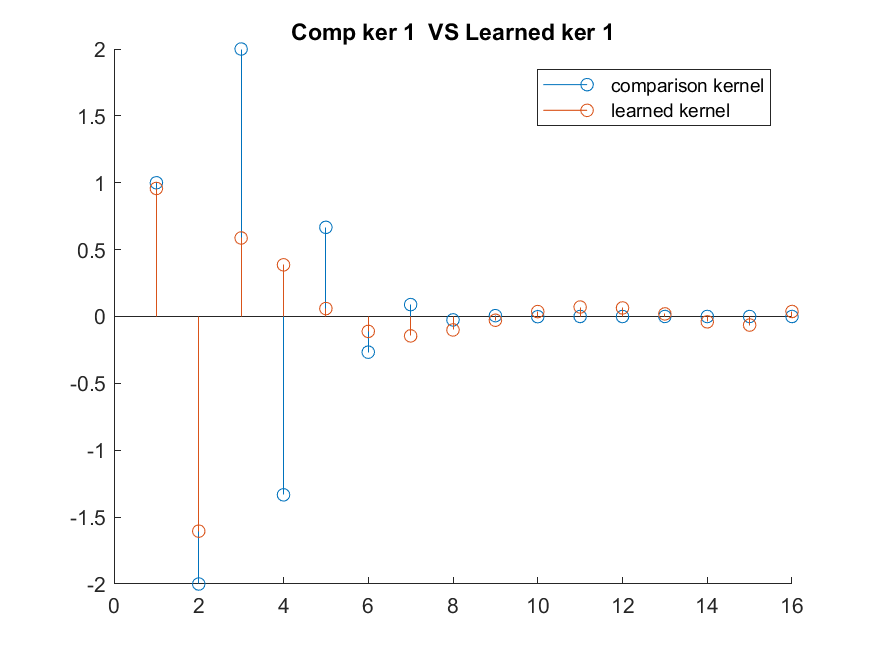
\includegraphics[width = \textwidth]{alphaHeat_noSmoothness_struct.png}
  \end{minipage}
  \vspace{10mm}
  \begin{minipage}[c]{.85\textwidth}
    \centering
    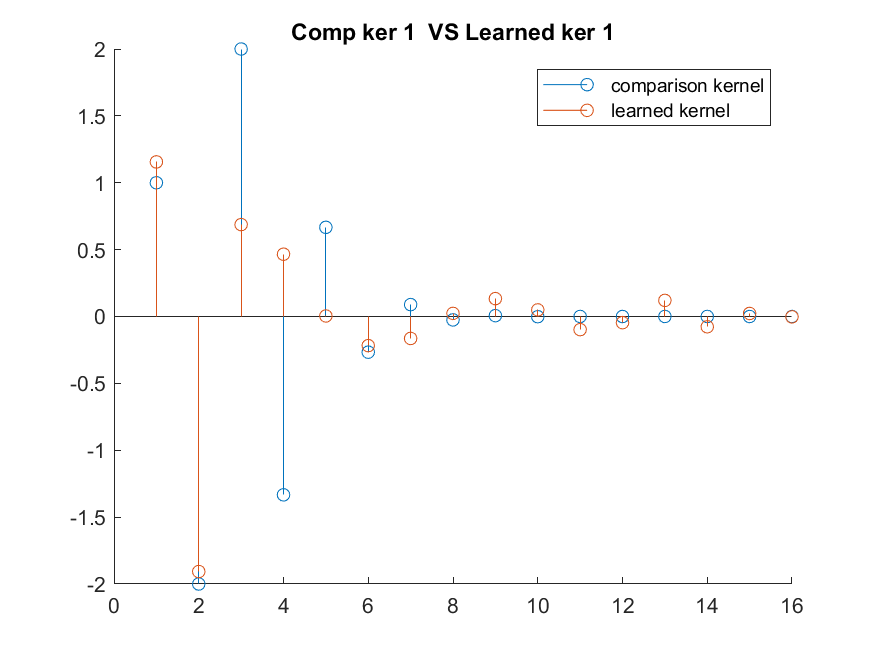
\includegraphics[width = \textwidth]{alphaHeat_Smoothness_struct.png}
  \end{minipage}
  \caption{Comparison between kernels coefficients without and with smoothness prior. Heat kernel   dataset}
  \label{fig:alphaHeat_struct}
\end{figure}

\begin{figure}[htbp]
  \centering
  \begin{minipage}[c]{.85\textwidth}
    \centering
    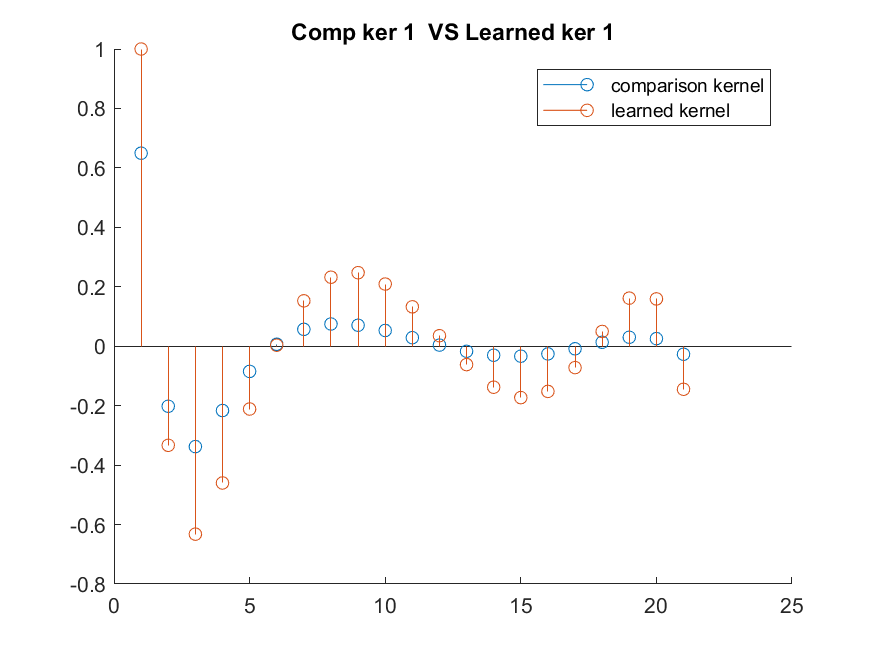
\includegraphics[width = \textwidth]{alphaDorina_noSmoothness_struct.png}
  \end{minipage}
  \vspace{10mm}
  \begin{minipage}[c]{.85\textwidth}
    \centering
    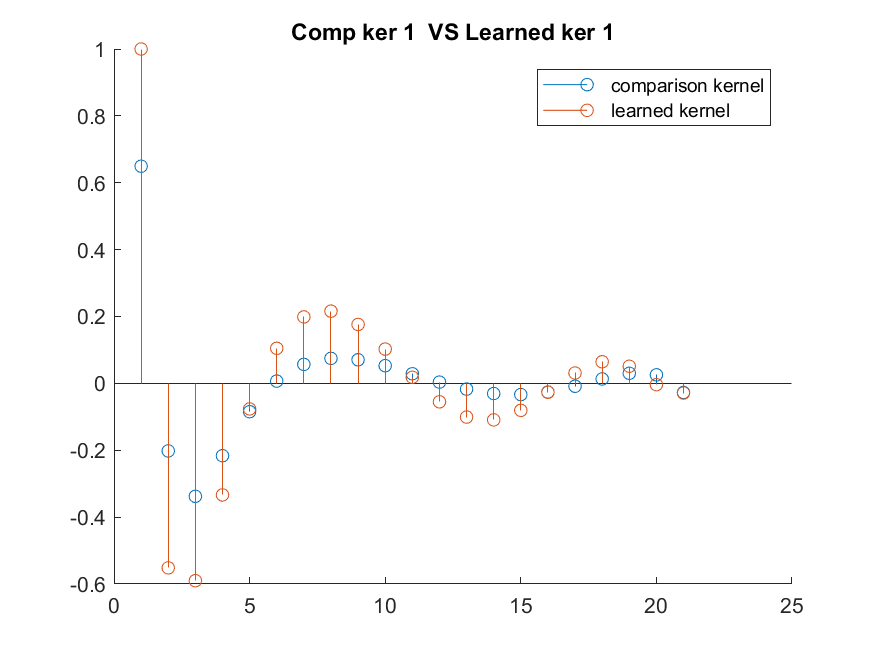
\includegraphics[width = \textwidth]{alphaDorina_Smoothness_struct.png}
  \end{minipage}
  \caption{Comparison between kernels coefficients without and with smoothness prior. Thanou et al.   dataset}
  \label{fig:alphaDorina_struct}
\end{figure}

\subsection{Second approach: smoothness in the constraints}
In the same way, here results show a general improvement, both regarding the reproduction error and the behavior of the kernel coefficients. In this case we can notice a slight improvement in both datasets concerning the reproduction error, \autoref{tab:errorHeat} and \autoref{tab:errorDorina} compare the results in the case with and without the smoothness prior, and show better results on average. One interesting thing that can be noticed is the stability of the learning process: adding the smoothness prior to the kernels has the consequence that the output values are stable during several iterations, while in the original algorithm there could be even some discrete variations.

\begin{table}[htbp]
  \centering
  \begin{tabular}{c|c|c}
    \multicolumn{1}{c|}{\textbf{Iteration number}} &
    \multicolumn{1}{c}{\textbf{Original algorithm}} &
    \multicolumn{1}{|c}{\textbf{Smoothness assumption}}\\
    \hline
    1 & 0.0250 & 0.0251\\
    2 & 0.0251 & 0.0251\\
    3 & 0.0250 & 0.0252\\
    4 & 0.0251 & 0.0248\\
    5 & 0.0251 & 0.0247\\
    \textbf{Average Error} & 0.02506 & 0.02498
  \end{tabular}
  \caption{Reproduction error comparison for the Heat kernel dataset}
  \label{tab:errorHeat}
\end{table}

\begin{table}[htbp]
  \centering
  \begin{tabular}{c|c|c}
    \multicolumn{1}{c|}{\textbf{Iteration number}} &
    \multicolumn{1}{c}{\textbf{Original algorithm}} &
    \multicolumn{1}{|c}{\textbf{Smoothness assumption}}\\
    \hline
    1 & 0.0217 & 0.0216\\
    2 & 0.0212 & 0.0215\\
    3 & 0.0213 & 0.0216\\
    4 & 0.0214 & 0.0216\\
    5 & 0.0213 & 0.0215\\
    \textbf{Average Error} & 0.02138 & 0.02156
  \end{tabular}
  \caption{Reproduction error comparison for the low frequency kernel from Thanou et al. dataset}
  \label{tab:errorDorina}
\end{table}

Moreover, making a comparison between the average computational cost we can see how the smoothness assumption improves the performance once again (\autoref{tab:CPUTime_dictionary}). Here, though, the difference is lower than in the previous approach, but this is comprehensible since now we are focusing on the constraints again, without reducing the number of actual unknown that the objective function is holding.

\begin{table}[htbp]
  \centering
  \begin{tabular}{c|c|c}
    &
    \multicolumn{1}{c}{\textbf{No smoothness assumption}} &
    \multicolumn{1}{|c}{\textbf{Smoothness assumption}}\\
    \hline
    \textbf{Heat Kernel dataset} & 0.9334 s & 0.1015 s\\
    \textbf{Thanou et al. dataset} & 0.1661 s & 0.1224 s\\
  \end{tabular}
  \caption{Computational cost comparison for the Heat kernel and the Thanou et al. kernel dataset}
  \label{tab:CPUTime_dictionary}
\end{table}

The improvement can also be noticed in the behavior of the kernels' coefficients: \autoref{fig:alphaHeatDictionary} represents another comparison between the values assumed by the original heat kernels' coefficients (blue lines), and the ones assumed by the learned coefficients in the case we are applying the smoothness prior or not. It can be seen how the coefficients in the case of no smoothness priors tend to have a less defined trend, while in the smoothness case they follow the original trend more faithfully. This aspect is shown even more clearly in the case of Thanou et al.'s dataset (\autoref{fig:alphaDorinaDictionary}), in which the coefficients have almost the same behavior, apart from their absolute value. The reason for this is mainly the nature of our constraints: in fact, since in the problem we are working with \gls{lmi},we are not imposing the solution of the optimization problem to be constrained to certain specific values, but to a range of them. As a consequence, the solution of the optimization process represents a point localized in a certain range.

\begin{figure}
  \centering
  \begin{minipage}[c]{.85\textwidth}
    \centering
    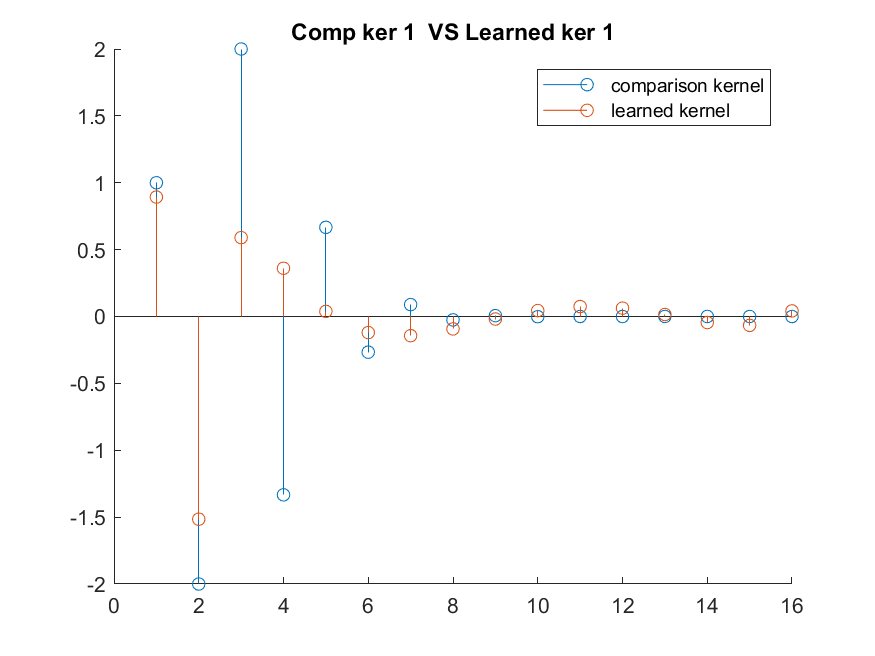
\includegraphics[width = \textwidth]{alphaHeat_noSmoothness_dictionary.png}
  \end{minipage}
  \vspace{10mm}
  \begin{minipage}[c]{.85\textwidth}
    \centering
    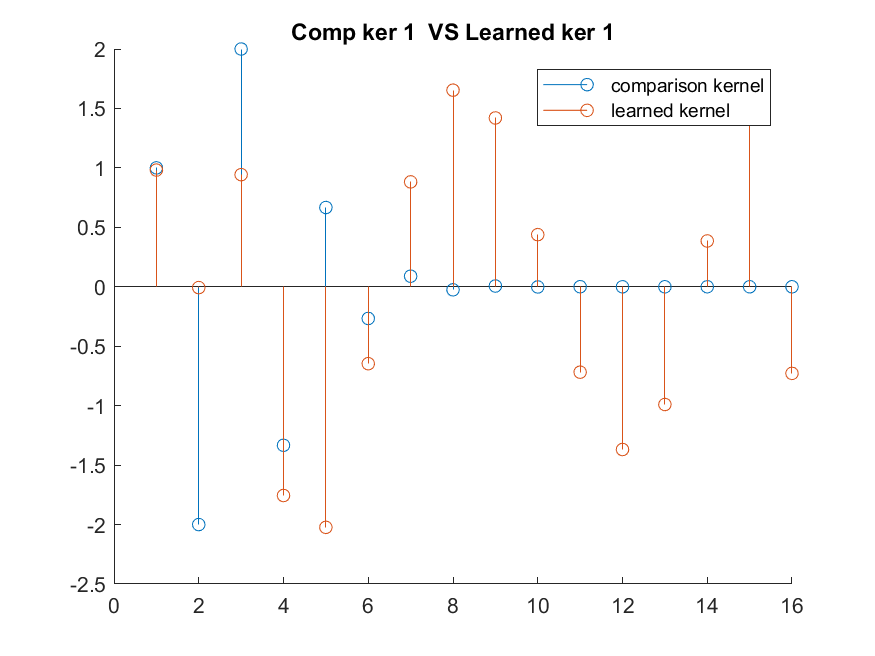
\includegraphics[width = \textwidth]{alphaHeat_Smoothness_dictionary.png}
  \end{minipage}
  \caption{Comparison between kernels coefficients without and with smoothness prior. Heat kernel   dataset}
  \label{fig:alphaHeatDictionary}
\end{figure}

\begin{figure}
  \centering
  \begin{minipage}[c]{.85\textwidth}
    \centering
    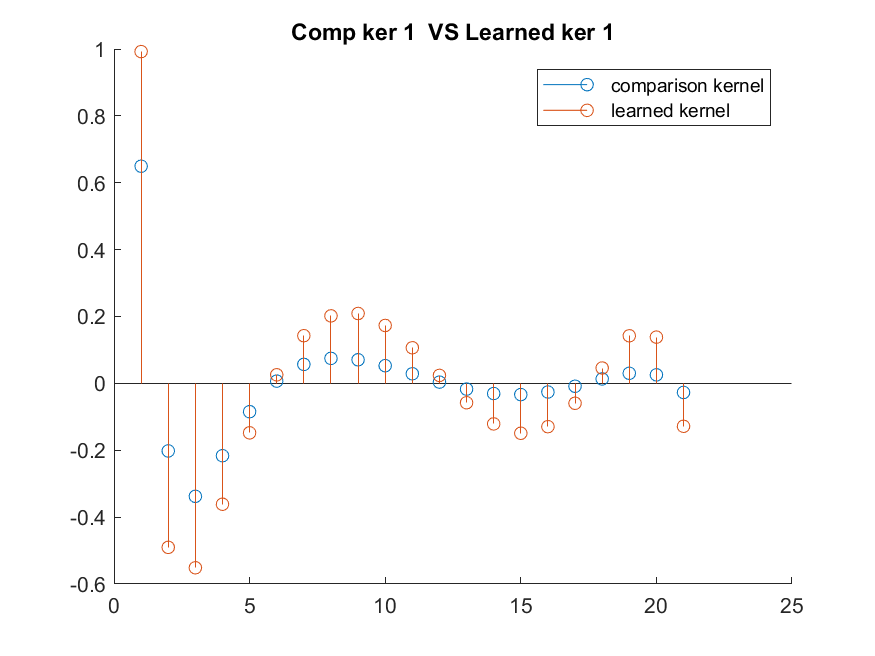
\includegraphics[width = \textwidth]{alphaDorina_noSmoothness_dictionary.png}
  \end{minipage}
  \vspace{10mm}
  \begin{minipage}[c]{.85\textwidth}
    \centering
    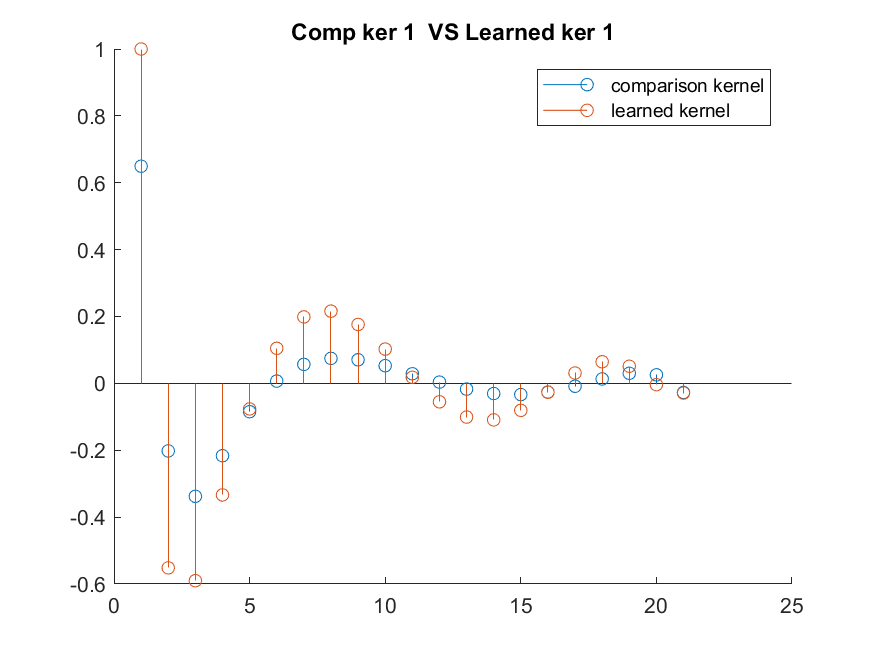
\includegraphics[width = \textwidth]{alphaDorina_Smoothness_dictionary.png}
  \end{minipage}
  \caption{Comparison between kernels coefficients without and with smoothness prior. Thanou et al. dataset}
  \label{fig:alphaDorinaDictionary}
\end{figure}


Finally, \autoref{fig:kernelHeatDictionary} and \autoref{fig:kernelDorinaDictionary} show the comparison between the original kernel and the learned kernel without and with smoothness prior in the case of a Heat kernel (\autoref{fig:kernelHeatDictionary}) and the dataset from  Thanou et al. (\autoref{fig:kernelDorinaDictionary}). It can be seen how the use of smoothness improves the overall trend also for the kernel shape, which is the ultimate purpose of the algorithm.

\begin{figure}[htbp]
  \begin{minipage}[c]{.5\textwidth}
    \centering
    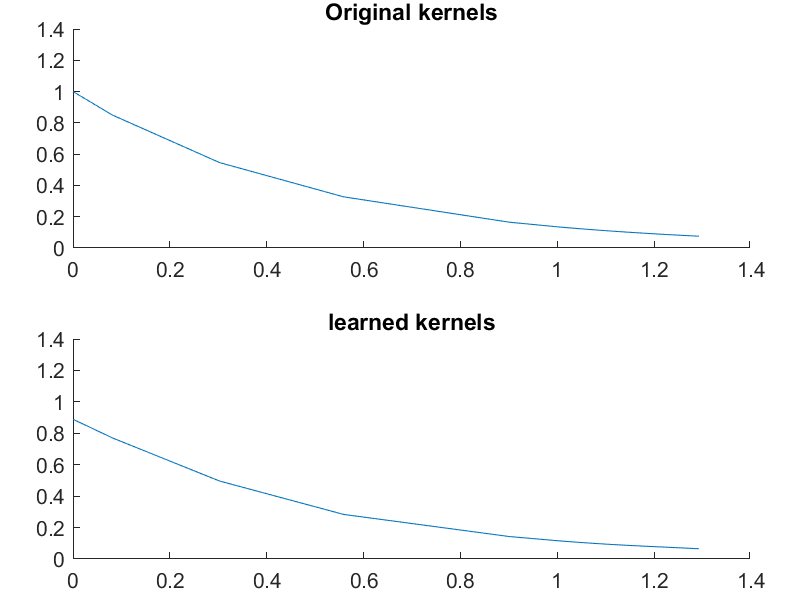
\includegraphics[width = .95\textwidth]{kernelHeat_noSmoothness_dictionary.png}
  \end{minipage}
  \begin{minipage}[c]{.5\textwidth}
    \centering
    \includegraphics[width = .95\textwidth]{kernelHeat_Smoothness_dictionary.png}
  \end{minipage}
  \caption{Comparison between kernels without and with smoothness prior. Heat kernel dataset}
  \label{fig:kernelHeatDictionary}
\end{figure}

\begin{figure}[htbp]
  \begin{minipage}[c]{.5\textwidth}
    \centering
    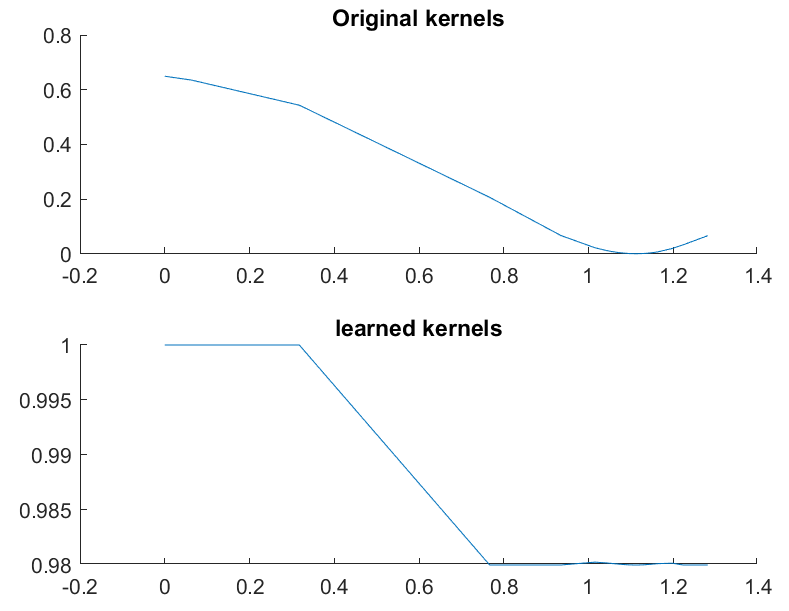
\includegraphics[width = .95\textwidth]{kernelDorina_noSmoothness_dictionary.png}
  \end{minipage}
  \begin{minipage}[c]{.5\textwidth}
    \centering
    \includegraphics[width = .95\textwidth]{kernelDorina_Smoothness_dictionary.png}
  \end{minipage}
  \caption{Comparison between kernels without and with smoothness prior. Thanou et al. kernel dataset}
  \label{fig:kernelDorinaDictionary}
\end{figure}

% Finally, if we look at the behavior of the CPU time necessary for every optimization step, we see that the values in the case we add our prior are in the same order of the ones obtained without it, which gives us further confirmation that out method, despite adding complexity due to the constraints, it does not, though, increase the computational cost.
%
% \begin{figure}
%   \begin{minipage}[c]{.5\textwidth}
%     \centering
%     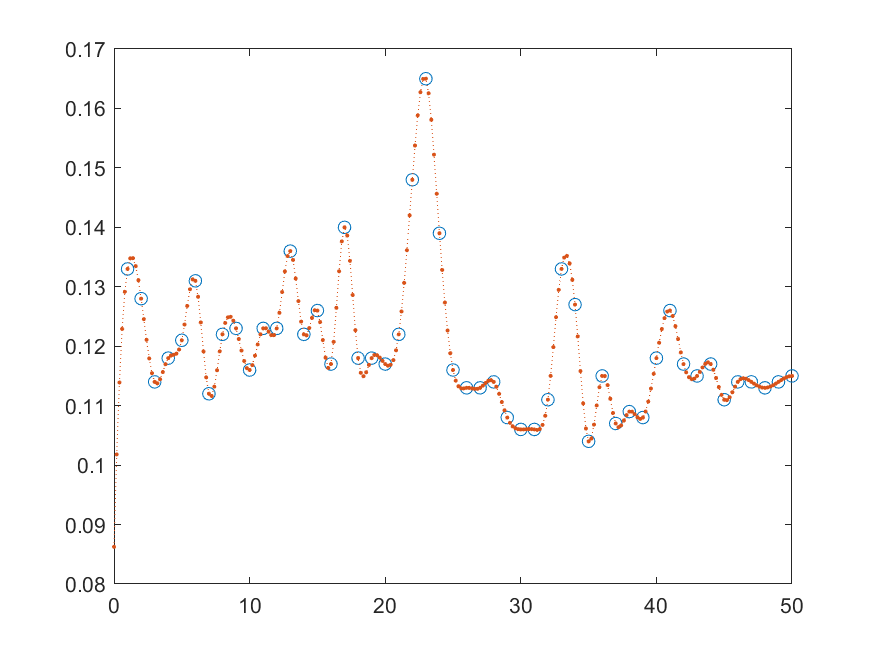
\includegraphics[width = \textwidth]{CPUHeat_noSmoothness_dictionary.png}
%   \end{minipage}
%   \begin{minipage}[c]{.5\textwidth}
%     \centering
%     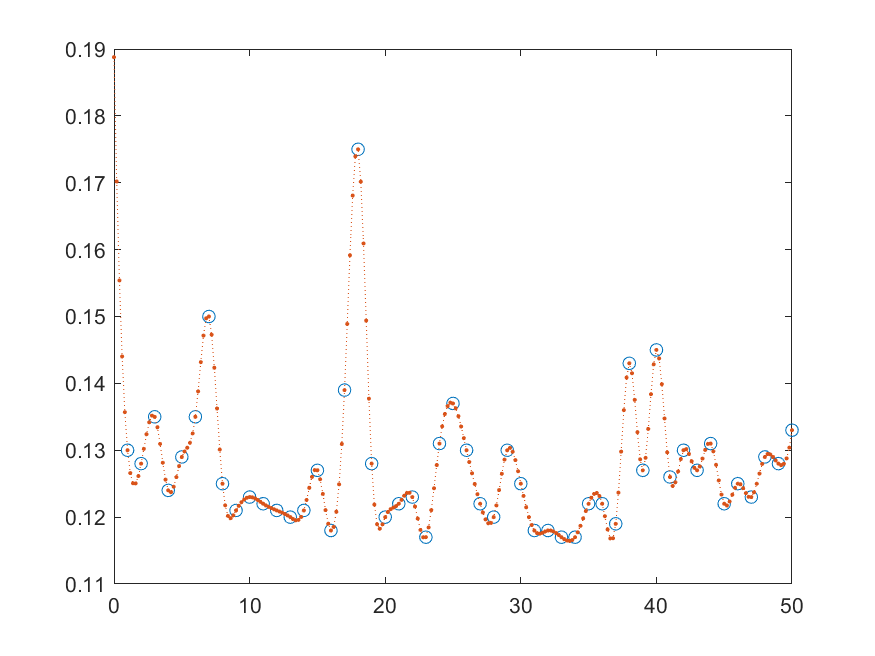
\includegraphics[width = \textwidth]{CPUHeat_Smoothness_dictionary.png}
%   \end{minipage}
%   \caption{Comparison between kernels without and with smoothness prior. Heat kernel dataset}
%   \label{fig:CPUHeatDictionary}
% \end{figure}
%
% \begin{figure}
%   \begin{minipage}[c]{.5\textwidth}
%     \centering
%     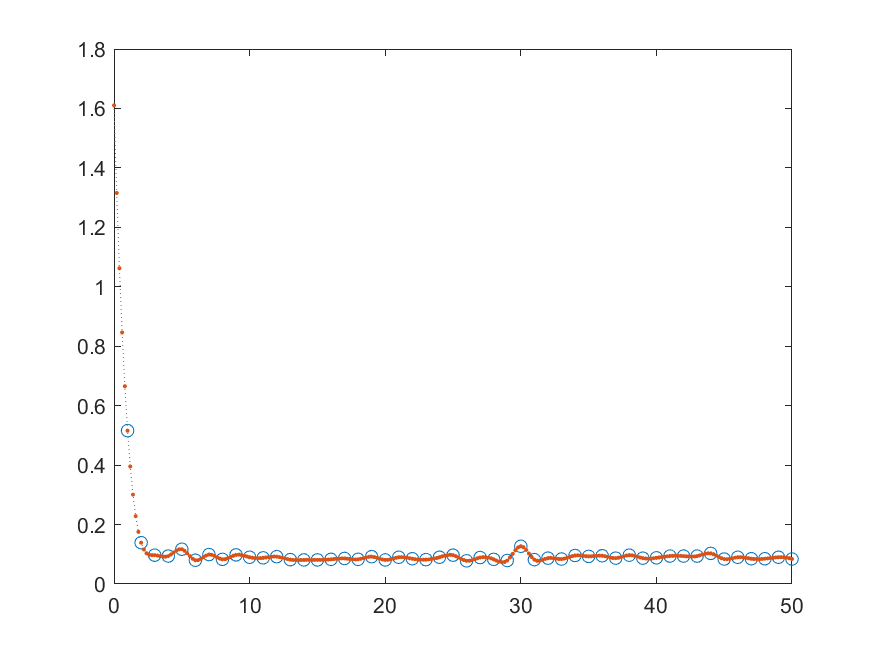
\includegraphics[width = \textwidth]{CPUDorina_noSmoothness_dictionary.png}
%   \end{minipage}
%     \begin{minipage}[c]{.5\textwidth}
%     \centering
%   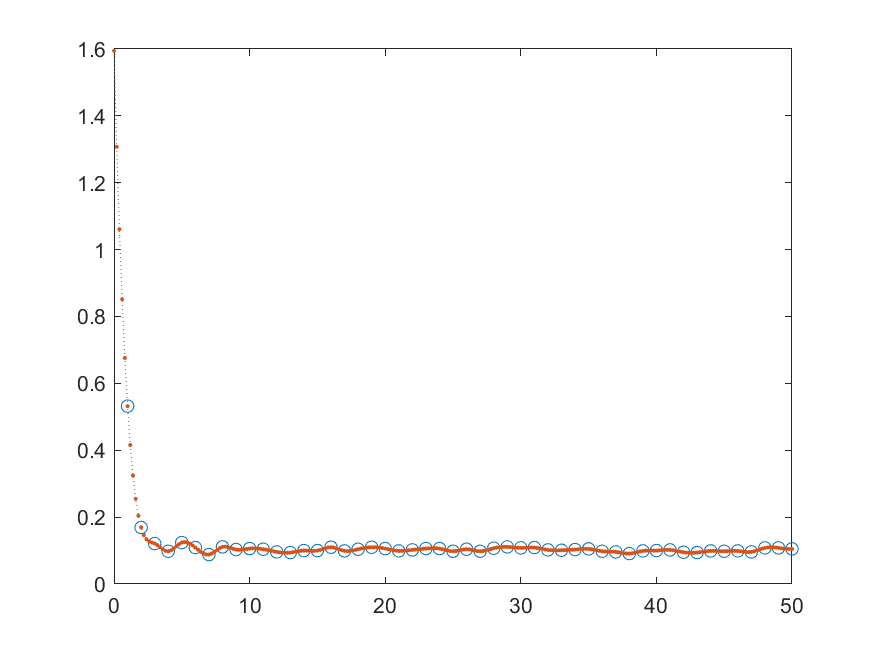
\includegraphics[width = \textwidth]{CPUDorina_Smoothness_dictionary.png}
%   \end{minipage}
%   \caption{Comparison between kernels without and with smoothness prior. Thanou et al. kernel dataset}
%   \label{fig:CPUDorinaDictionary}
% \end{figure}
